\scanpage{114}
% L01--02. The first margin rule is brown-toned; its maker is unassigned.
\margin{\figure{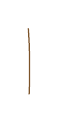
\begin{tikzpicture}\draw[brown!65!black,line width=.45pt] (0,0) .. controls (.02,-.25) and (.02,-.65) .. (.01,-.84);\end{tikzpicture}}}
est de plus propre, alors pour \uline{toute} sous-variété linéaire $\inserted{L_t}$ de codimensio\handwritten{n}
$s$, $Y_t=f_t^{-1}(L_t)$ est géométriquement connexe.

% L03--04.
Conjuguant avec 2, on trouve, par l'argument qui a permis de
déduire 3 de 1 :

% L05--07; the marginal reference is on two slanted lines.
\margin{\handwritten{\begin{tabular}{@{}l@{}}cf.\\S\unsure{C|G}A 1 X \unsure{2,11|2.11|2,II|2.II}\end{tabular}}}
\margin{\figure{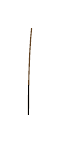
\begin{tikzpicture}\draw[brown!50!black,line width=.4pt] (.04,0) .. controls (.01,-.3) and (0,-.7) .. (0,-1.1);\draw[black,line width=.55pt] (0,-.72)--(0,-1.1);\end{tikzpicture}}}
\uline{Corollaire} 5: \deleted{Avec}\inserted{\handwritten{Sous}} les hypothèses de \unsure{3|4}, \inserted{avec $X$ propre,} l'homomorphisme danonique
$\handwritten{\pi}_1(Y_{\bar t})\handwritten{\rightarrow}\handwritten{\pi}_1(X)$ ($\handwritten{\simeq}\handwritten{\pi}_1(X_{\bar t})$ par le théorème de changement de base) est
surjectif.

% L08--11.
Nous désirons également un énoncé analogue à 5, donnant une surjectivité pour des $\handwritten{\pi}_1$ pour un $t$ non générique, mais sans hypothèse de propreté, et pour des quotients plus gros du $\handwritten{\pi}_1$ que ceux envisagés dans (**).
On peut\deleted{\unsure{nt|nl}} donner à ce sujet le résultat suivant:

% L12--15. Mixed typewriter cells are not assigned a correction chronology.
\margin{\figure{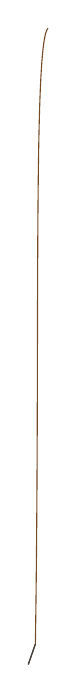
\begin{tikzpicture}\draw[brown!60!black,line width=.4pt] (.16,0) .. controls (-.03,-.18) and (.06,-4) .. (0,-7.82) --(-.09,-8.08);\draw[black!75,line width=.45pt] (0,-7.82)--(-.09,-8.08);\end{tikzpicture}}}
\uline{Théorème} 6. Su\unsure{p|i}\unsure{p|t}osons $k$ algébriquement clos, \inserted{\handwritten{et}} $X$ propre, $f:X\handwritten{\rightarrow}P^r$, \deleted{et}
le sous -espace linéaire $L_t$ de $P^r$ de codimension $s$ (défini sur $k$, pour
fixer les idées) \deleted{tels qu'on ait} et enfin le sous-schéma fermé $D$ de $X$
tels qu'on ait ceci; \deleted{où on a posé $U=X-D$}

% L16.
a) \deleted{$U_t=U\unsure{\cap}X_t$ et} $\deleted{X}\handwritten{Y}_t=f^{-1}(L_t)$ est non vide.

% L17--18.
b) Pour tout $x\handwritten{\in}\deleted{X}\handwritten{Y}_t$, $X$ est lisse en $x$, $Y_t$ est lisse en $x$\handwritten{,} de
codime\unsure{n|m|t}sion $s$ dans $X$ en $x$, $f$ est net en $x$.

% L19--21.
c) Pour tout $x\handwritten{\in}D_t=D\handwritten{\cap}Y_t$, o\deleted{\`{}}u \deleted{bien} bien $\operatorname{codim}_x(D_t,\deleted{\unsure{T|X}}\handwritten{Y}_t)\handwritten{\geqslant}2$, ou bien
$D_{\deleted{\unsure{t}}}$ est un diviseur \unsure{e|s}\unsure{n|u}r $X$ en $x$ et $\deleted{D_t}$ induit sur $Y_t$ en $x$ un diviseur
à croisements normaux.
% Two small points lie immediately below-left of the corrected Y in codim, not in the margin.
\figure{\begin{tikzpicture}[x=1cm,y=1cm]\fill[black!75] (0,0) circle (.014);\fill[black] (-.035,-.16) circle (.016);\end{tikzpicture}}

% L22--28. The first p in Supposons inherits the p|i doubt at L12.
Supposons $U=X-D$ irréductible, et considérons l'inclusion $U_t=U\handwritten{\cap}Y_t$
$\handwritten{\longrightarrow}U$. \deleted{Alors $U_t$} Soit $\handwritten{\pi}_1^t(U)$ le \deleted{grou} quotient du groupe fondamental de
$U$ \deleted{formé des} qui classifie les revêtements de $U$ qui sont modérément
ramifiés en les composantes irréductibles de codimension 1 de $D$ dans $X$
qui rencontrent $Y_t$, \deleted{(\unsure{i.e.} telles que $D$} et $\overset{\unsure{t}}{\handwritten{\pi}}_1^t(\unsure{U|V}_t)$ le quotient \deleted{analogue} de
$\handwritten{\pi}_1(U_t)$ qui classifie les revêtements qui sont modérément ramifiés en
les composantes irréductibles de codimension 1 de $D_t$. On a un homomor-%
% archive sheet number: 113
